





% \subsubsection{The resulting rooms}

% Please add the following required packages to your document preamble:
% \usepackage{graphicx}
% Please add the following required packages to your document preamble:
% \usepackage{graphicx}


% Please add the following required packages to your document preamble:
% \usepackage{graphicx}
% \begin{table*}[]
% \resizebox{\textwidth}{!}{%
% \begin{tabular}{|l|lllll|l|llllll|}
% \hline
% User & Len       & Lin       & Meso      & Spatial   & Symmetry  & Fitness   & $W_{dens}$ & $W_{spar}$ & $E_{dens}$ & $E_{spar}$ & $T_{dens}$ & $T_{spar}$ \\ \hline
% 1    & 0.6±0.1   & 0.92±0.05 & 0.06±0.08 & 0.49±0.24 & 0.55±0.23 & 0.74±0.07 & 0.42±0.11  & 0.22±0.09  & 0.17±0.12  & 0.19±0.16  & 0.14±0.12  & 0.13±0.15  \\
% 2    & 0.59±0.18 & 0.92±0.02 & 0.17±0.14 & 0.36±0.12 & 0.36±0.25 & 0.72±0.07 & 0.23±0.05  & 0.16±0.03  & 0.33±0.09  & 0.28±0.14  & 0.34±0.11  & 0.41±0.24  \\
% 3    & 0.6±0.21  & 0.9±0.04  & 0.17±0.1  & 0.38±0.21 & 0.54±0.16 & 0.71±0.11 & 0.29±0.11  & 0.21±0.08  & 0.25±0.0   & 0.33±0.1   & 0.33±0.12  & 0.33±0.01  \\
% 4    & 0.58±0.17 & 0.92±0.02 & 0.11±0.13 & 0.42±0.19 & 0.33±0.32 & 0.7±0.12  & 0.23±0.06  & 0.14±0.02  & 0.27±0.04  & 0.32±0.07  & 0.35±0.08  & 0.41±0.02  \\
% 5    & 0.54±0.13 & 0.92±0.02 & 0.17±0.14 & 0.39±0.18 & 0.48±0.22 & 0.7±0.1   & 0.24±0.05  & 0.2±0.07   & 0.34±0.18  & 0.27±0.14  & 0.43±0.17  & 0.42±0.13  \\
% 6    & 0.52±0.13 & 0.92±0.03 & 0.14±0.12 & 0.37±0.19 & 0.33±0.12 & 0.66±0.1  & 0.25±0.08  & 0.18±0.04  & 0.33±0.06  & 0.32±0.07  & 0.31±0.04  & 0.37±0.05  \\
% 7    & 0.58±0.14 & 0.9±0.02  & 0.11±0.08 & 0.24±0.08 & 0.32±0.26 & 0.73±0.15 & 0.2±0.02   & 0.18±0.02  & 0.26±0.03  & 0.33±0.07  & 0.29±0.07  & 0.36±0.07  \\
% 8    & 0.66±0.1  & 0.91±0.02 & 0.11±0.08 & 0.28±0.08 & 0.12±0.13 & 0.89±0.05 & 0.14±0.05  & 0.17±0.03  & 0.21±0.1   & 0.33±0.19  & 0.46±0.28  & 0.31±0.18  \\ \hline
% avg  & 0.58±0.03 & 0.91±0.01 & 0.13±0.03 & 0.37±0.06 & 0.38±0.11 & 0.73±0.05 & 0.25±0.06  & 0.18±0.02  & 0.27±0.05  & 0.29±0.04  & 0.33±0.08  & 0.34±0.07  \\ \hline
% \end{tabular}%
% }
% \caption{Summary of the created rooms filtered by each user. The first five values relates to the MAP-Elites dimensions, then the fitness of the rooms, and finally density and sparsity values for wall (W), enemies (E), and treasures (T).}
% \label{tab:peruser}
% \end{table*}



% Please add the following required packages to your document preamble:
% \usepackage{graphicx}
\begin{table}[]
\resizebox{\columnwidth}{!}{%
\begin{tabular}{|l|lll|}
\hline
     & AI replaced & Human replaced & Interactions \\ \hline
AIv1 & 3.31±2.1     & 1.63±1.47       & 3.88±0.59    \\
AIv2 & 24.94±6.67   & 12.06±5.29      & 8.56±3.28    \\
AIv3 & 19.25±5.13   & 0               & 9.13±3.64    \\ \hline
\end{tabular}%
}
\caption{Summary of the interactions between AI and human}
\label{tab:humanai-interactions}
\end{table}



\subsection{Results}

% We present the results from the user study regarding the final designed rooms, the room design process with the AI, and the participant's interview responses. Figure~\ref{fig:human-ai-contribution} and~\ref{fig:human-ai-tiletypes} show the tile contribution for both human and AI per room and tested version, and the final tile distribution across all versions, respectively. Figure~\ref{fig:userdesigned-rooms} shows a sample\footnote{The first room designed by the first five testers} of the designed rooms corresponding to the different AI versions, respectively. 

% The designed rooms when interacting with the AIv1 (fig.~\ref{fig:userdesigned-rooms}.a) generally include a vast majority of human-placed tiles or unedited tiles, as shown by the low amount of pink tinted tiles and fig.~\ref{fig:human-ai-contribution}.a. Many of the rooms display treasures and enemies placed close to each other, often with an enemy blocking a treasure. As displayed in fig.~\ref{fig:userdesigned-rooms}.b, when interacting with the AIv2, rooms contain more AI edited tiles and long continuous walls are less common compared to when using AIv1. Fig.~\ref{fig:userdesigned-rooms}.c shows a sample of the designs using AIv3. The resulting rooms are less symmetric, contain less continuous walls, and are in general, somewhat less organized. Based on fig.~\ref{fig:human-ai-contribution}.c, the divide of tiles placed by the two co-creators is largely close to even.

% The relation between the total amount of tiles placed by the human designer and the AI for each version provides insight into how much the human designers incorporated the AI in their design process, as well as how this varied in the different versions. As expected, the amount of tiles remaining at the end design increased as the AI got more initiative. When using AIv1, the human designers generally contributed with a majority of tiles to the resulting room (86\% in general). When using AIv2, the results vary more between rooms and/or designers such as fig.~\ref{fig:userdesigned-rooms}.b 1 and 9 with a general 49\% of tiles placed by the human designer. In AIv3, the AI generally had a majority of tiles in the resulting rooms (32\% placed tiles by human designers in general). Figure~\ref{fig:human-ai-tiletypes} gives insight into the differences in the design processes and choices between co-creators. The human designer focuses mostly on adding walls, creating structures and shapes, while the AI designer focuses on removing tiles for floors aiming mainly at breaking structures and adding meso-patterns.

We present the results from the user study regarding the designed rooms, the room design process with the AI, and the participant's interview responses. Figure~\ref{fig:human-ai-contribution} and~\ref{fig:human-ai-tiletypes} show the tile contribution for both human and AI per room and tested version, and the final tile distribution across all versions, respectively. Figure~\ref{fig:userdesigned-rooms} shows a sample of the designed rooms corresponding to the different AI versions, respectively. 

The designed rooms, when interacting with the AIv1 (fig.~\ref{fig:userdesigned-rooms}.a), generally include a vast majority of human-placed tiles or unedited tiles (86\%). Many of the rooms display treasures and enemies placed close to each other, often with an enemy blocking a treasure. As displayed in fig.~\ref{fig:userdesigned-rooms}.b (AIv2), rooms contain more AI edited tiles (51\%), and long continuous walls are less common compared to when using AIv1. Fig.~\ref{fig:userdesigned-rooms}.c shows a sample of the designs using AIv3. The resulting rooms are less symmetric, contain fewer continuous walls, and are, in general, somewhat less organized. 

The relation between the total amount of tiles placed by the human designer and the AI for each version provides insight into how much the human designers incorporated the AI in their design process. When using AIv1, the human designers generally contributed with a majority of tiles to the resulting room (86\% in general). When using AIv2, the results vary more between rooms and/or designers, such as fig.~\ref{fig:userdesigned-rooms}.b 1 and 9 with a general 49\% of tiles placed by humans. In AIv3, the AI generally had a majority of tiles in the resulting rooms (32\% placed tiles by human designers in general). Figure~\ref{fig:human-ai-tiletypes} shows the tiles by each co-creator. Whereas human designers focused mostly on walls and structures, the AI focused on removing tiles and adding floors. 

%Furthermore, table~\ref{tab:peruser} and~\ref{tab:AIavgValues} summarizes the created rooms by users and AI versions, respectively. In general, there is not much variation among users

Furthermore, table~\ref{tab:AIavgValues} and~\ref{tab:humanai-interactions} summarizes the created rooms by AI version. Table~\ref{tab:AIavgValues} shows that there is not much variation regarding the IC MAP-Elites dimensions, but Symmetry and Meso patterns reduce as the AI gains more agency, and there are fewer spatial patterns in the high and low agency. It also shows that wall and enemy density and sparsity go lower and higher, respectively. This is expected, given that as the AI is more dominant in the design (fig.~\ref{fig:human-ai-contribution}), walls are diminished (fig.~\ref{fig:human-ai-tiletypes}), which can also be observed in the examples in fig.~\ref{fig:userdesigned-rooms}. Finally, designers spent less time on their design for AIv1 and AIv3. In AIv1,  designers can edit rooms towards their goal and the AI does not modify their design (unless wanted), which means that the designer does not need to modify the room much. This is expected to increase for AIv2 and AIv3 because the AI now adds its editions, which count towards the steps. However, since the AI can add as many tiles as the designer, the designer is still doing roughly half of the steps. When using AIv3, rooms take slightly fewer steps than AIv2, probably due to the AI taking over areas where to design and designers trying to work around constraints further discussed in the next section. 

Table~\ref{tab:humanai-interactions} shows the interaction between human and AI. As expected, the human designers interacted less with the AI in AIv1, and in general, they overwrote less since they could decide which elements from the AI to include. Five out of the 16 rooms included AI-placed tiles where the human designer did not replace any of the AI tiles. Interactions and human and AI tile replacements increase for AIv2 and AIv3, which is also expected. The AI overwrote an avg. of 24.94 and 19.25 tiles in each subsequent version, and human designers overwrote an avg. of 12.06 in AIv2. This shows that the AI had more involvement and changed the design more often. The human designer could either use their turn to replace the tiles or continue using those tiles. However, in AIv2, the designers did not replace all of the AI tiles; instead, they also chose to work around them and replaced them when needed, allowing the AI to participate more. In 13 out of the 16 rooms created the designer replaced fewer tiles than the AI did, and for 9 of those it was less than 50\%.

%which shows that the 

%There are five rooms that included AI placed tiles where the human designer did not replace any of the AI tiles.


%(5 rooms included AI placed tiles that the human designe. 

%As expected, the AI overwrite less and the interactions are 

%Finally, designers spent less time in their design for AIv1 and AIv3. In AIv1, given that designers can edit the rooms towards their goal and the AI do not modify their design (unless wanted), the designer does not need to modify much the room. This is expected to increase for AIv2 and AIv3 because the AI now adds their editions, which counts towards the steps. However, given that the AI can add as many tiles as the designer, the designer is still only doing half of the steps. When using AIv3, rooms take slightly less steps than AIv2, probably due to the AI taking over areas where to design and designers trying to work around constraints further discussed in the next section. 

%only adding around half of the tiles .

%In AIv3, given both that designers had to fix 


% that human designers focused mostly on wall

% Figure~\ref{fig:human-ai-tiletypes} gives insight into the differences in the design processes and choices between co-creators. The human designer focuses mostly on adding walls and creating structures, while the AI designer focuses on removing tiles for floors breaking structures and adding meso-patterns.


% , with only one case not following this trend (see Figure 12).
% When using AIv2, the results vary more between rooms and/or designers (see Figure 12). As shown in Figure 9, examples of this variation is room 1 and 2, which are created by participant 1, with a very low percentage of AI placed tiles in the resulting room, compared to room 4 with around 90\% AI-placed tiles, or 11 with 100\% AI-placed tiles. 
% When using AIv3, the AI generally had a majority of tiles in the resulting rooms (see Figure 14).

% Reviewing the relation between the amount of tiles placed by both co-creators in the resulting rooms for each version provides an understanding of how much each co-creator influenced the final product, and how this varies in the different versions. 
% When using AIv1, the human designers generally contributed with a majority of tiles to the resulting room, with only one case not following this trend (see Figure 12).
% When using AIv2, the results vary more between rooms and/or designers (see Figure 12). As shown in Figure 9, examples of this variation is room 1 and 2, which are created by participant 1, with a very low percentage of AI placed tiles in the resulting room, compared to room 4 with around 90\% AI-placed tiles, or 11 with 100\% AI-placed tiles. 
% When using AIv3, the AI generally had a majority of tiles in the resulting rooms (see Figure 14).

% The split between between human placed tiles and AI-placed tiles for all resulting rooms using each versions show a less detailed and more general appreciation of the influence on the final products between co-creators. With this compilation, the human designers contributed with a significant majority of the tiles of the resulting rooms compared to AIv1 (see Figure 15). When using AIv2, the split between co-creators is very close to even (see Figure 16). When using AIv3, the AI contributed with the majority of tiles (see Figure 17).

% \subsubsection{Types of tiles placed}

% The amount of the different types of tiles that the  human designers used, the difference between the same statistics for the AI, gives insight into the differences in the design processes and choices between co-creators. 

% As seen in Figure 18, the most common type of tiles placed by human designer sin descending order is wall, treasure, enemy, floor and boss. Comparing this to the AI's most commonly placed tiles displayed in Figure 19, there is a notable difference. The most common tiles placed by AI in descending order is floor, treasure, and finally wall and enemy on the same percentage. The AI did not place down any boss tiles. None of the versions of AI deviated from the collective division of tile-types in a notable way.


% The first design vary in their design, however many of them contain continuous walls of lengths above 2 tiles.
% The first rooms vary in their design, however many of them contain continuous walls of lengths above 2 tiles.a room containing a boss as their second room when using the AI with low initiative.

% As displayed in Figure 7, the resulting rooms when using the AI with medium initiative include half the amount of bosses compared to Figure 6. The rooms that do include bosses are always the second room produced by the participant. Long continuous walls are slightly less common compared to when using the AI with lower initiative. Similarly to the results of using AIv1, symmetry is identified in some of the rooms produced with AIv2, for example Room 2 and room 10. Compared to Figure 6, the rooms produced contain more pink tinted tiles in Figure 7. The amount of pink tiles vary greatly, with only one tile in Room 1 and 70 tiles in Room 11.

% As displayed in Figure 8, the least amount of bosses where present in the resulting rooms when using the AI with high initiative. Additionally, long continuous walls is the least common when using AIv3. Symmetry is slightly less frequent compared to the resulting rooms from the other version of AI, with only Room 2 and 6 with apparent symmetry. The divide of tiles placed by the two co-creators is largely close to even.

\begin{figure}[h]
 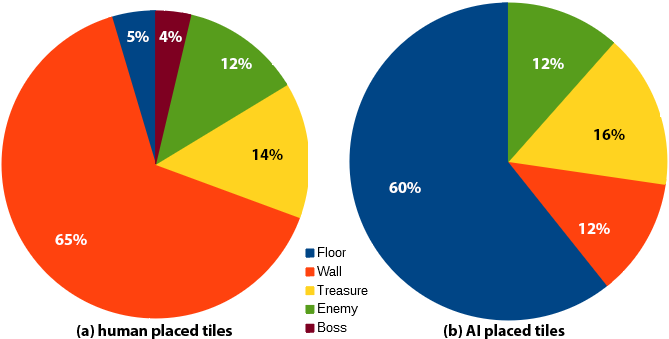
\includegraphics[width=\columnwidth]{images/combined_tile_types.png}
 \caption{The types of tiles placed and their percentage of occurrence by human designers (a) and the AI (b)}
 \label{fig:human-ai-tiletypes}
\end{figure}

\subsubsection{Perceptions of the different AI versions}

Four participants preferred to use AIv1 due to higher controllability over the final design. Two participants preferred AIv2 since they liked the efficiency of the AI placing down tiles, but they still remained in control over the design process. One participant said that they preferred both AIv1 and AIv3, as they felt that they fulfilled different purposes. AIv1 contributed with inspiration to get out of a writers block kind-of situation in level design, while AIv3 offered a more unusual creative experience, and created unique levels. One participant preferred AIv3 categorizing it as more efficient. However, AIv3 was the most disliked due to most participants feeling constrained by the AI's decisions, which forced themto workaround the AI's design; too invasive on their design process, and in general, feeling the AI dismissed their contributions. Two participants disliked AIv2 the most due to frustration and slowing their design process because of the repetitive work of recreating their original idea as the AI would overwrite their tiles. One participant disliked AIv1 as it was the slowest to work with.

\subsubsection{AI's behavior}

\begin{figure*}[h]
 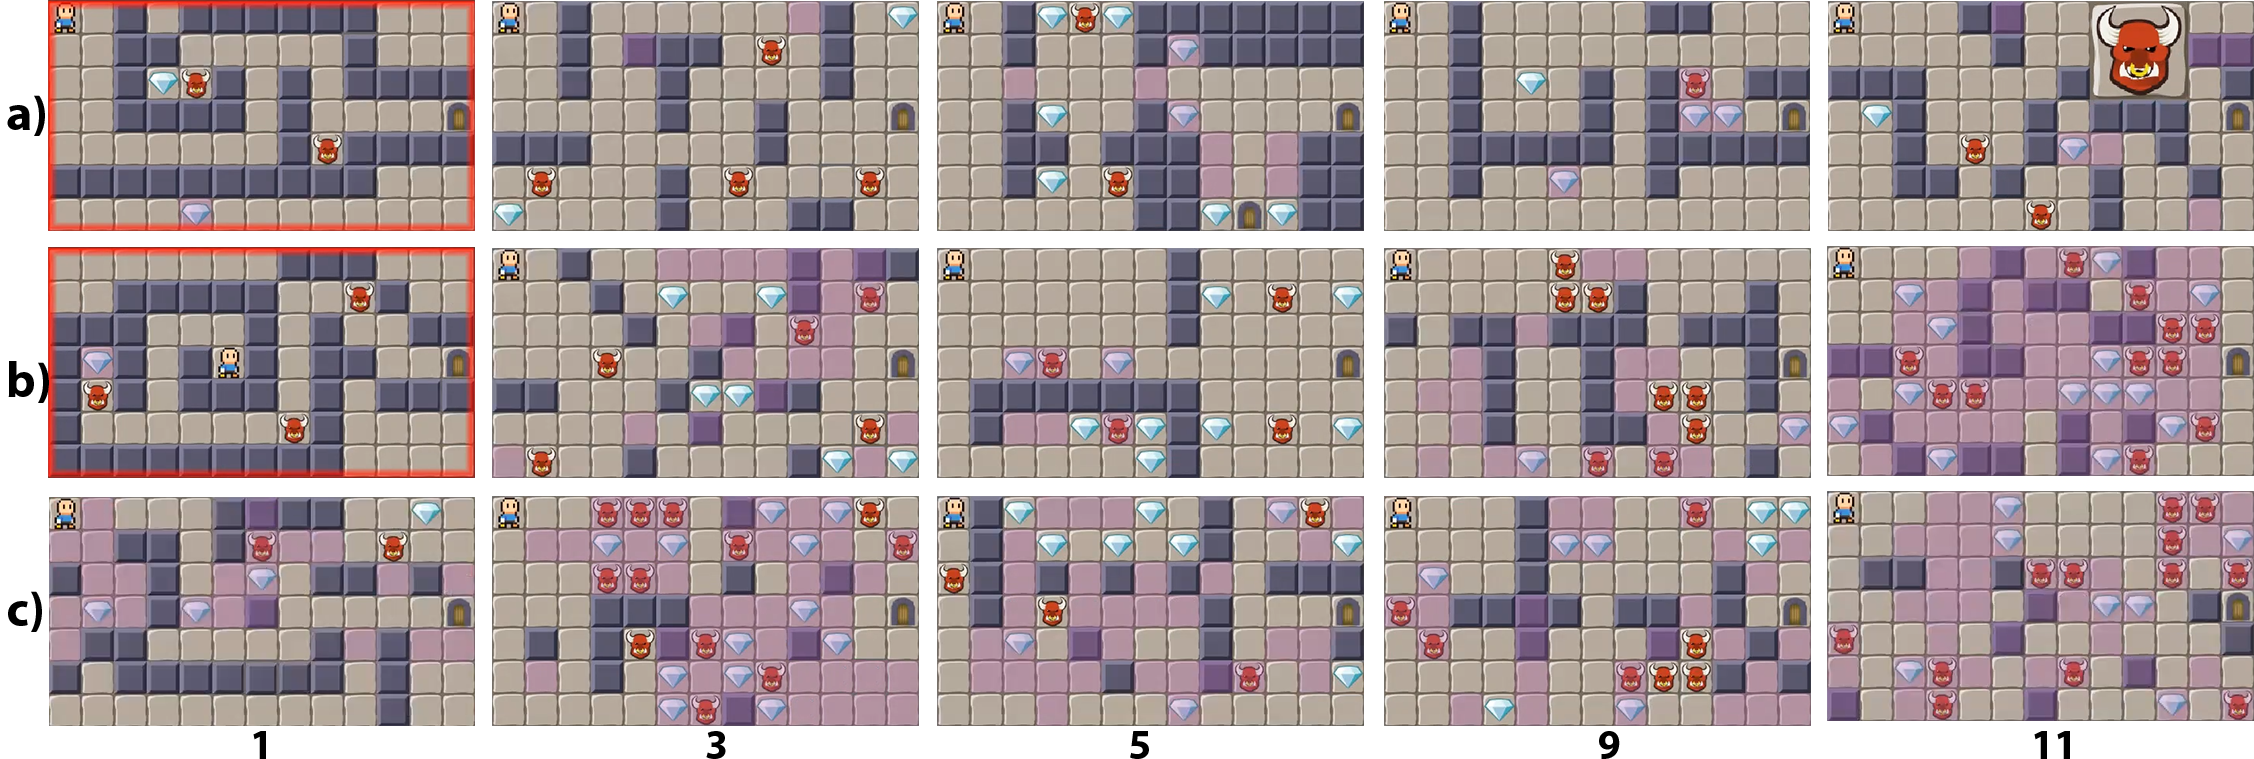
\includegraphics[width=\textwidth]{images/rooms-designed-1.png}
 \caption{Sample resulting rooms from the study. a, b, and c are samples from the same users using the different versions. Red borders indicate that the room contains unreachable tiles. Purple tinted tiles are the ones added by the AI.}
 \label{fig:userdesigned-rooms}
\end{figure*}

Five participants described the AI's behavior as random and unpredictable. Many mentioned that the AI often placed floor tiles over the human-placed walls, treasures, enemies, and bosses. Additionally, two participants mentioned that the AI often broke down sub-rooms or long walls with floor tiles. The more positive descriptions of the AI's behavior were that the AI repaired their level if it had unreachable tiles by placing floor tiles on the positions wall tiles were, making all tiles reachable. One participant expressed that they thought the AI created unique-looking high-quality levels.

\subsubsection{The Creative Relationship}

Five participants expressed that the AI contributed with ideas they liked and either kept or considered incorporating. Many also expressed that they found it frustrating that the AI overwrote the human placed walls, treasures, enemies, or boss tiles with floor tiles, as they perceived this as the AI removing their contributions without adding anything new. All participants answered that they did adapt to AIv2 and AIv3 during their design process. When using AIv2, the participants adapted to the AI by either being inspired by the AI's contribution or by getting frustrated with the AI repeatedly placing tiles the human designer did not like. When using AIv3, they felt they had to adjust to whatever the AI contributed and felt forced to adapt. Additionally, six participants answered that they did not feel that the AI adapted to them. One answered that it did feel that the AI adapted to them, and one participant had no opinion. 

Four participants described the relationship as working together with someone who only says no to your ideas without contributing to new ideas. Three participants described it as frustrating and/or a fight for control between the AI and the human designer. Two participants described it as an iterative collaboration and compared it to two people working on the same product but in different steps. One participant described the relationship as a brainstorming session where you work in a ``Yes, and..." fashion, meaning you work iteratively and only adds to the idea and never decline the other collaborator's contribution. 

% Many of the participants, five out of eight, expressed that the AI contributed with ideas that they liked and either kept or considered incorporating. Many also expressed that they found it frustrating that the AI overwrote the human placed walls, treasures, enemies or boss-tiles with floor-tiles, as they perceived this as the AI removing their contributions without adding anything new. Another common answer was that AIv3 was very frustrating for them to work with. 

% All eight participants answered that they did adapt to the AI during their design process. The participants did not adapt when using AIv1.However, when using AIv2, the participants adapted to the AI by either being inspired by the AI's contribution, or by getting frustrated with the AI repeatedly placing tiles the human designer did not like. When using AIv3 in particular, the participants expressed that they had to adjust to whatever the AI contributed with, and that they felt forced to adapt.
% Additionally, the majority, six out of eight participants, answered that they did not feel that the AI adapted to them. One answered that it did feel that the AI adapted to them, and one participant had no opinion.


% Four of the participants described the relationship between the AI and the human designer as working together with someone who only says no to your ideas, without contributing with new ideas. Three participants described it as frustrating and/or a fight for control between the AI and the human designer. Two of the participants described it as an iterative collaboration, and compared it to two people working on the same product, but in different steps. One participant described the relationship as a brainstorm session where you work in a "Yes, and..." fashion, meaning you work iteratively  and only adds to the idea, and never declines the other collaborators contribution. 

\subsubsection{The Creative Process}

Four participants mentioned that the AI negatively affected their creative process, especially when the AI placed floor tiles over their placed walls, treasures, enemies, and bosses. This was described by multiple participants as the AI ``destroying their creations", and many felt forced to let the AI ``take control over the room." Two participants described the creative process as the AI and the human designer working against each other. Two other participants described it as a process where the AI brought forward ideas that they found interesting. One participant described it as letting the AI form an idea that the human designer finally polished. 

\subsubsection{Constraints and Design Goals}

Five participants answered they felt progressively more constrained as the AI gained more control, although one participant answered that they did not feel constrained at all with any of the versions. Six participants answered they had a design goal of creating a boss room. However, the AI placed floor tiles over the boss tiles, making this impossible in AIv2 and AIv3, forcing them to change their design goals. Two participants answered that they did not have set design goals and solely created content each turn with no specific concept for the whole room in mind.

% A majority of participants, five out of eight, answered that they felt progressively more constrained as the AI gained more control. One participant answered that they felt constrained when using the AI with medium initiative(AIv2), but not with the other versions. One Participant answered that they did not feel constrained at all, with any of the versions.

% Six out of eight participant answered that they had a design goal of creating a boss room, however the AI placed floor-tiles over the boss-tiles, making this impossible in AIv2 and AIv3, forcing them to change their design goals. Two participants answered that they did not have set design goals, and solely created content each turn with no specific concept for the whole room in mind.


% \subsubsection{Answers to the interview questions}

% Each subsection summarizes the answers to the set of questions from the interview which are designed to relate to a specific concern in the study.


% \emph{The perceptions of the different versions of AI (Q1, Q2)}


% Many of the participants, four out of eight, preferred to use the AI with low initiative (AIv1). The reasoning was that the participants preferred to have full control over the design. The second most preferred version of AI is the one with medium initiative, AIv2, from two out of eight participants. The reason they chose AIv2, was that they liked the efficiency of the AI placing down tiles, but they still remained in control over the design process.
% One participant said that they preferred both AIv1 and AIv3, and felt that they fulfilled different purposes; AIv1 contributed with inspiration to get out of a writers block kind of situation in level design, while AIv3 offered a more unusual creative experience, and created unique levels.
% Only one participant preferred the AI with high initiative (AIv3), with the motivation that it was efficient.


% The AI with the highest initiative was the most disliked.  Motivations to this was that they were constrained by the AI's decisions, that it was too invasive on their design process, and that they were forced to work around what the AI designed.
% Two participants answered that they disliked working with AIv2 the most, because the AI would overwrite the human designers tiles during its round, and the human would then spend their turn to recreate the original idea again. They felt this was a back and forth that was frustrating and slowed down the design process.
% One participant answered that they disliked the AI with low initiative the most, as it was the slowest to work with in their opinion.



% \emph{The Behaviour of the AI (Q4)}


% A majority of participants, five out of eight, described the behaviour of the AI as random and unpredictable. Many mentioned that they noticed the AI often placed floor-tiles over the human-placed walls, treasures, enemies and bosses. Additionally, two out of eight participants mentioned that the AI often broke down sub-rooms or long walls by placing floor tiles. The more positive descriptions of the AI's behaviour were that the AI repaired their level if it had unreachable tiles by placing floor-tiles on the positions wall-tiles were, making all tiles reachable. One participant expressed that they thought the AI created unique-looking levels of high quality.


% \emph{The Creative Relationship (Q3, Q6, Q7, Q8)}


% Many of the participants, five out of eight, expressed that the AI contributed with ideas that they liked and either kept or considered incorporating. Many also expressed that they found it frustrating that the AI overwrote the human placed walls, treasures, enemies or boss-tiles with floor-tiles, as they perceived this as the AI removing their contributions without adding anything new. Another common answer was that AIv3 was very frustrating for them to work with. 


% All eight participants answered that they did adapt to the AI during their design process. The participants did not adapt when using AIv1.However, when using AIv2, the participants adapted to the AI by either being inspired by the AI's contribution, or by getting frustrated with the AI repeatedly placing tiles the human designer did not like. When using AIv3 in particular, the participants expressed that they had to adjust to whatever the AI contributed with, and that they felt forced to adapt.
% Additionally, the majority, six out of eight participants, answered that they did not feel that the AI adapted to them. One answered that it did feel that the AI adapted to them, and one participant had no opinion.


% Four of the participants described the relationship between the AI and the human designer as working together with someone who only says no to your ideas, without contributing with new ideas. Three participants described it as frustrating and/or a fight for control between the AI and the human designer. Two of the participants described it as an iterative collaboration, and compared it to two people working on the same product, but in different steps. One participant described the relationship as a brainstorm session where you work in a "Yes, and..." fashion, meaning you work iteratively  and only adds to the idea, and never declines the other collaborators contribution. 


% \emph{The Creative Process (Q9)}


% Four participants mentioned that their creative process was negatively affected by the AI, namely when the AI placed floor tiles over human placed walls, treasures, enemies and bosses. This was described by multiple participants as the AI "destroying their creations", and many felt forced to let the AI "take control over the room". Two participants described the creative process as the AI and the human designer working against each other. Two participants described it as a process where the AI brought forward ideas that they found interesting. One participant described it as letting the AI form an idea, that the human designer finally polished. 




% \emph{Constraints (Q5)}


% A majority of participants, five out of eight, answered that they felt progressively more constrained as the AI gained more control. One participant answered that they felt constrained when using the AI with medium initiative(AIv2), but not with the other versions. One Participant answered that they did not feel constrained at all, with any of the versions.


% \emph{Design Goals (Q10)}


% Six out of eight participant answered that they had a design goal of creating a boss room, however the AI placed floor-tiles over the boss-tiles, making this impossible in AIv2 and AIv3, forcing them to change their design goals. Two participants answered that they did not have set design goals, and solely created content each turn with no specific concept for the whole room in mind.


%This section presents the results gathered from the user study in the form of automatically collected user data from the tool, as well as qualitative data in the form of participants answers to the interview questions. The quantitative data is used to analyse the contributions made by both agents and their differences and relations, in an effort to highlight discussion points and offer insight necessary to answer the research questions. The qualitative data is used to explore opinions of the tool, the AI, and the co-creative process. Comments made when using the system and the answers and discussions collected from the interview provide valuable insight, that can be used when attempting to answer the research questions.


% \begin{figure*}[t]
%  \includegraphics[width=\textwidth]{images/LOW_COMBINED.png}
%  \caption{All of the resulting rooms when using AIv1.}
% \end{figure*}

% \subsubsection{The resulting rooms}


% The rooms produced during the user study are displayed in Figure 6, 7 and 8. Rooms with red borders are infeasible, meaning there are unreachable tiles. The UI displays a warning when this happens, and the AI can repair this during its turn, however the resulting rooms that are infeasible are a result of the human designer creating unreachable areas, and then immediately selecting to go to the World Editing view, before pressing "End Turn". 
% Each participant created two rooms for each version of the AI. Participant 1 created Room 1 and Room 2 for all version, Participant 2 created Room 3 and Room 4 for all version, etc. All of the participants had the option to adjust the sizes of the rooms in the World Editing view before entering the Room Editing view, however none of them did, and therefore all of the resulting rooms are of the default size. The designer also has the option to change the location of the hero and the doors. The location of the hero was only moved twice in all of the session, and the doors where never moved. 


% \emph{AIv1}

% As displayed in Figure 6, all of the participants created a room containing a boss as their second room when using the AI with low initiative. Bosses tend to be placed in the right side of the room. Many of the second rooms also contain a number of treasure-tiles at the far right. 
% Many of the rooms display treasures and enemies placed close to each other, often with an enemy blocking a treasure. Some of the rooms display a prominent symmetry, for example Room 4 and Room 10.
% The first rooms vary in their design, however many of them contain continuous walls of lengths above 2 tiles. The rooms generally include a vast majority of human-placed tiles or unedited tiles, as shown by the low amount of pink tinted tiles. 


% \emph{AIv2}

% As displayed in Figure 7, the resulting rooms when using the AI with medium initiative include half the amount of bosses compared to Figure 6. The rooms that do include bosses are always the second room produced by the participant. Long continuous walls are slightly less common compared to when using the AI with lower initiative. Similarly to the results of using AIv1, symmetry is identified in some of the rooms produced with AIv2, for example Room 2 and room 10.
% Compared to Figure 6, the rooms produced contain more pink tinted tiles in Figure 7. The amount of pink tiles vary greatly, with only one tile in Room 1 and 70 tiles in Room 11.


% \emph{AIv3}

% As displayed in Figure 8, the least amount of bosses where present in the resulting rooms when using the AI with high initiative. Additionally, long continuous walls is the least common when using AIv3. Symmetry is 
% slightly less frequent compared to the resulting rooms from the other version of AI, with only Room 2 and 6 with apparent symmetry. The divide of tiles placed by the two co-creators is largely close to even.



% % \begin{figure*}[t]
% %  \includegraphics[width=\textwidth]{images/MEDIUM_COMBINED.png}
% %  \caption{All of the resulting rooms when using AIv2.}
% % \end{figure*}
 
% % \begin{figure*}
% %  \includegraphics[width=\textwidth]{images/HIGH_COMBINED.png}
% %  \caption{All of the resulting rooms when using AIv3.}
% % \end{figure*}

% \subsubsection{Amounts of tiles placed per co-creator}

% The relation between the total amount of tiles placed by the human designer and the AI for each version provides insight into how much the human designers incorporated the AI in their design process, as well as how this varied in the different versions.
% The collected data show that the relation between the total amount of tiles placed by the human designer and the AI vary. When using the AI with low initiative (AIv1), humans placed a significant majority of the tiles (see Figure 9).  
% When using the AI with medium initiative (AIv2) the relation is more varied, with a slight majority of human placed tiles overall (see Figure 10).
% When using the the AI with high initiative (AIv3) the relation between the amount of tiles placed by human and amount of tiles placed by the AI  is the most even out of the three, with one case of the human allowing the AI to place almost three times as many tiles as himself (see Figure 11).

% % \begin{figure}
% %     \includegraphics[width=\columnwidth]{images/Quantitative Data/low_tiles_placed_by.png}
% %     \caption{The amount of tiles placed by both co-creators when using AIv1.}
% %     \label{fig:my_label}
% % \end{figure}

% % \begin{figure}
% %     \includegraphics[width=\columnwidth]{images/Quantitative Data/medium_tiles_placed_by.png}
% %     \caption{The amount of tiles placed by both co-creators when using AIv2.}
% %     \label{fig:my_label}
% % \end{figure}

% % \begin{figure}[b]
% %     \includegraphics[width=\columnwidth]{images/Quantitative Data/high_tiles_placed_by.png}
% %     \caption{The amount of tiles placed by both co-creators when using AIv3.}
% %     \label{fig:my_label}
% % \end{figure}

% \subsubsection{Tiles placed per co-creator in the resulting rooms}

% Reviewing the relation between the amount of tiles placed by both co-creators in the resulting rooms for each version provides an understanding of how much each co-creator influenced the final product, and how this varies in the different versions. 
% When using AIv1, the human designers generally contributed with a majority of tiles to the resulting room, with only one case not following this trend (see Figure 12).
% When using AIv2, the results vary more between rooms and/or designers (see Figure 12). As shown in Figure 9, examples of this variation is room 1 and 2, which are created by participant 1, with a very low percentage of AI placed tiles in the resulting room, compared to room 4 with around 90\% AI-placed tiles, or 11 with 100\% AI-placed tiles. 
% When using AIv3, the AI generally had a majority of tiles in the resulting rooms (see Figure 14).

% % \begin{figure}
% %     \includegraphics[width=\columnwidth]{images/Quantitative Data/low_final_tiles_bar.png}
% %     \caption{The percentage of tiles per co-creator in the resulting rooms when using AIv1.}
% %     \label{fig:my_label}
% % \end{figure}

% % \begin{figure}
% %     \includegraphics[width=\columnwidth]{images/Quantitative Data/medium_final_tiles_bar.png}
% %     \caption{The percentage of tiles per co-creator in the resulting rooms when using AIv2.}
% %     \label{fig:my_label}
% % \end{figure}

% % \begin{figure}
% %     \includegraphics[width=\columnwidth]{images/Quantitative Data/high_final_tiles_bar.png}
% %     \caption{The percentage of tiles per co-creator in the resulting rooms when using AIv3.}
% %     \label{fig:my_label}
% % \end{figure}

% The split between between human placed tiles and AI-placed tiles for all resulting rooms using each versions show a less detailed and more general appreciation of the influence on the final products between co-creators. With this compilation, the human designers contributed with a significant majority of the tiles of the resulting rooms compared to AIv1 (see Figure 15). When using AIv2, the split between co-creators is very close to even (see Figure 16). When using AIv3, the AI contributed with the majority of tiles (see Figure 17).


% % \begin{figure}[h!]
% %     \includegraphics[width=\columnwidth]{images/Quantitative Data/low_final_tiles_pie.png}
% %     \caption{The percentage of tiles per co-creator in all resulting rooms when using AIv1.}
% %     \label{fig:my_label}
% % \end{figure}

% % \begin{figure}[h!]
% %     \includegraphics[width=\columnwidth]{images/Quantitative Data/medium_final_tiles_pie.png}
% %     \caption{The percentage of tiles per co-creator in all resulting rooms when using AIv2.}
% %     \label{fig:my_label}
% % \end{figure}

% % \begin{figure}[h!]
% %     \includegraphics[width=\columnwidth]{images/Quantitative Data/high_final_tiles_pie.png}
% %     \caption{The percentage of tiles per co-creator in all resulting rooms when using AIv3.}
% %     \label{fig:my_label}
% % \end{figure}


% \subsubsection{Types of tiles placed}

% The amount of the different types of tiles that the  human designers used, the difference between the same statistics for the AI, gives insight into the differences in the design processes and choices between co-creators. 

% % \begin{figure}[h!]
% %     \includegraphics[width=\columnwidth]{images/Quantitative Data/Human_Tile_Types.png}
% %     \caption{The types of tiles placed by human designers and their percentage of occurrence.}
% %     \label{fig:my_label}
% % \end{figure}

% % \begin{figure}[h!]
% %     \includegraphics[width=\columnwidth]{images/Quantitative Data/AI_Tile_Types.png}
% %     \caption{The types of tiles placed by all versions of AI and their percentage of occurrence.}
% %     \label{fig:my_label}
% % \end{figure}

% As seen in Figure 18, the most common type of tiles placed by human designer sin descending order is wall, treasure, enemy, floor and boss. Comparing this to the AI's most commonly placed tiles displayed in Figure 19, there is a notable difference. The most common tiles placed by AI in descending order is floor, treasure, and finally wall and enemy on the same percentage. The AI did not place down any boss tiles. None of the versions of AI deviated from the collective division of tile-types in a notable way.





% \emph{Suggestions of Improvements (Q11)}


% All participants suggested removing the constrain of turns and amount of tiles per turn. Three participants suggested that the AI could be used more as an assistant to the human designer, by giving the AI parameters such as area or type of tiles to place. Three participants suggested using a more intelligent or human-like AI-agent. Examples of how the AI could be improved included valuing the types of tiles similarly to how the human designer does, learning from what the human contributes with and adapting its behaviour, and possibly attempting to predict the design goal that the human designer has. One participant answered that they would like to have the AI suggest complete generated rooms, that the human designer can then polish or edit freely. One participant had a related suggestion, which is a final step of the design process when the room is complete, where the human can edit an additional set amount of tiles, giving the human a chance to overwrite some AI-placed tiles.
















